\documentclass[11pt, a4paper]{report}

\usepackage[dutch]{babel}
\usepackage{booktabs}
\usepackage{caption}
\usepackage{fancyhdr}
\usepackage{graphicx}
\usepackage{hyperref}
\usepackage{longtable}
\usepackage{lastpage}
\usepackage{ragged2e}
\usepackage{titlepic}
\usepackage{xcolor}
\usepackage{xstring}

\hypersetup{
	colorlinks=true,
	linkcolor=blue,
	filecolor=magenta,
	urlcolor=cyan,
	pdftitle={KEIKO Document by KAT},
}

\definecolor{box-color-critical}{HTML}{42145F}
\definecolor{box-color-high}{HTML}{D6293E}
\definecolor{box-color-medium}{HTML}{C36100}
\definecolor{box-color-low}{HTML}{00519C}
\definecolor{box-color-recommendation}{HTML}{C3DDF6}
\definecolor{box-color-unknown}{HTML}{FFFFFF}
\definecolor{box-color-pending}{HTML}{FFFFFF}

\definecolor{color-critical}{HTML}{FFFFFF}
\definecolor{color-high}{HTML}{FFFFFF}
\definecolor{color-medium}{HTML}{FFFFFF}
\definecolor{color-low}{HTML}{FFFFFF}
\definecolor{color-recommendation}{HTML}{000000}
\definecolor{color-unknown}{HTML}{000000}
\definecolor{color-pending}{HTML}{000000}

%KEIKO-specific variables
\newcommand\application{KEIKO 0.0.1.dev1}
\newcommand\reporttitle{Bevindingenrapport voor Organisatie Rieven}
\newcommand\tlp{AMBER}
\newcommand\tlpbox{\colorbox{black}{\color{orange}TLP:AMBER}}
\newcommand\humanreadable[1]{\protect\StrSubstitute{\empty#1}{|}{ | }}
%END-KEIKO

\pagestyle{fancy}

\fancypagestyle{plain}{
	\cfoot{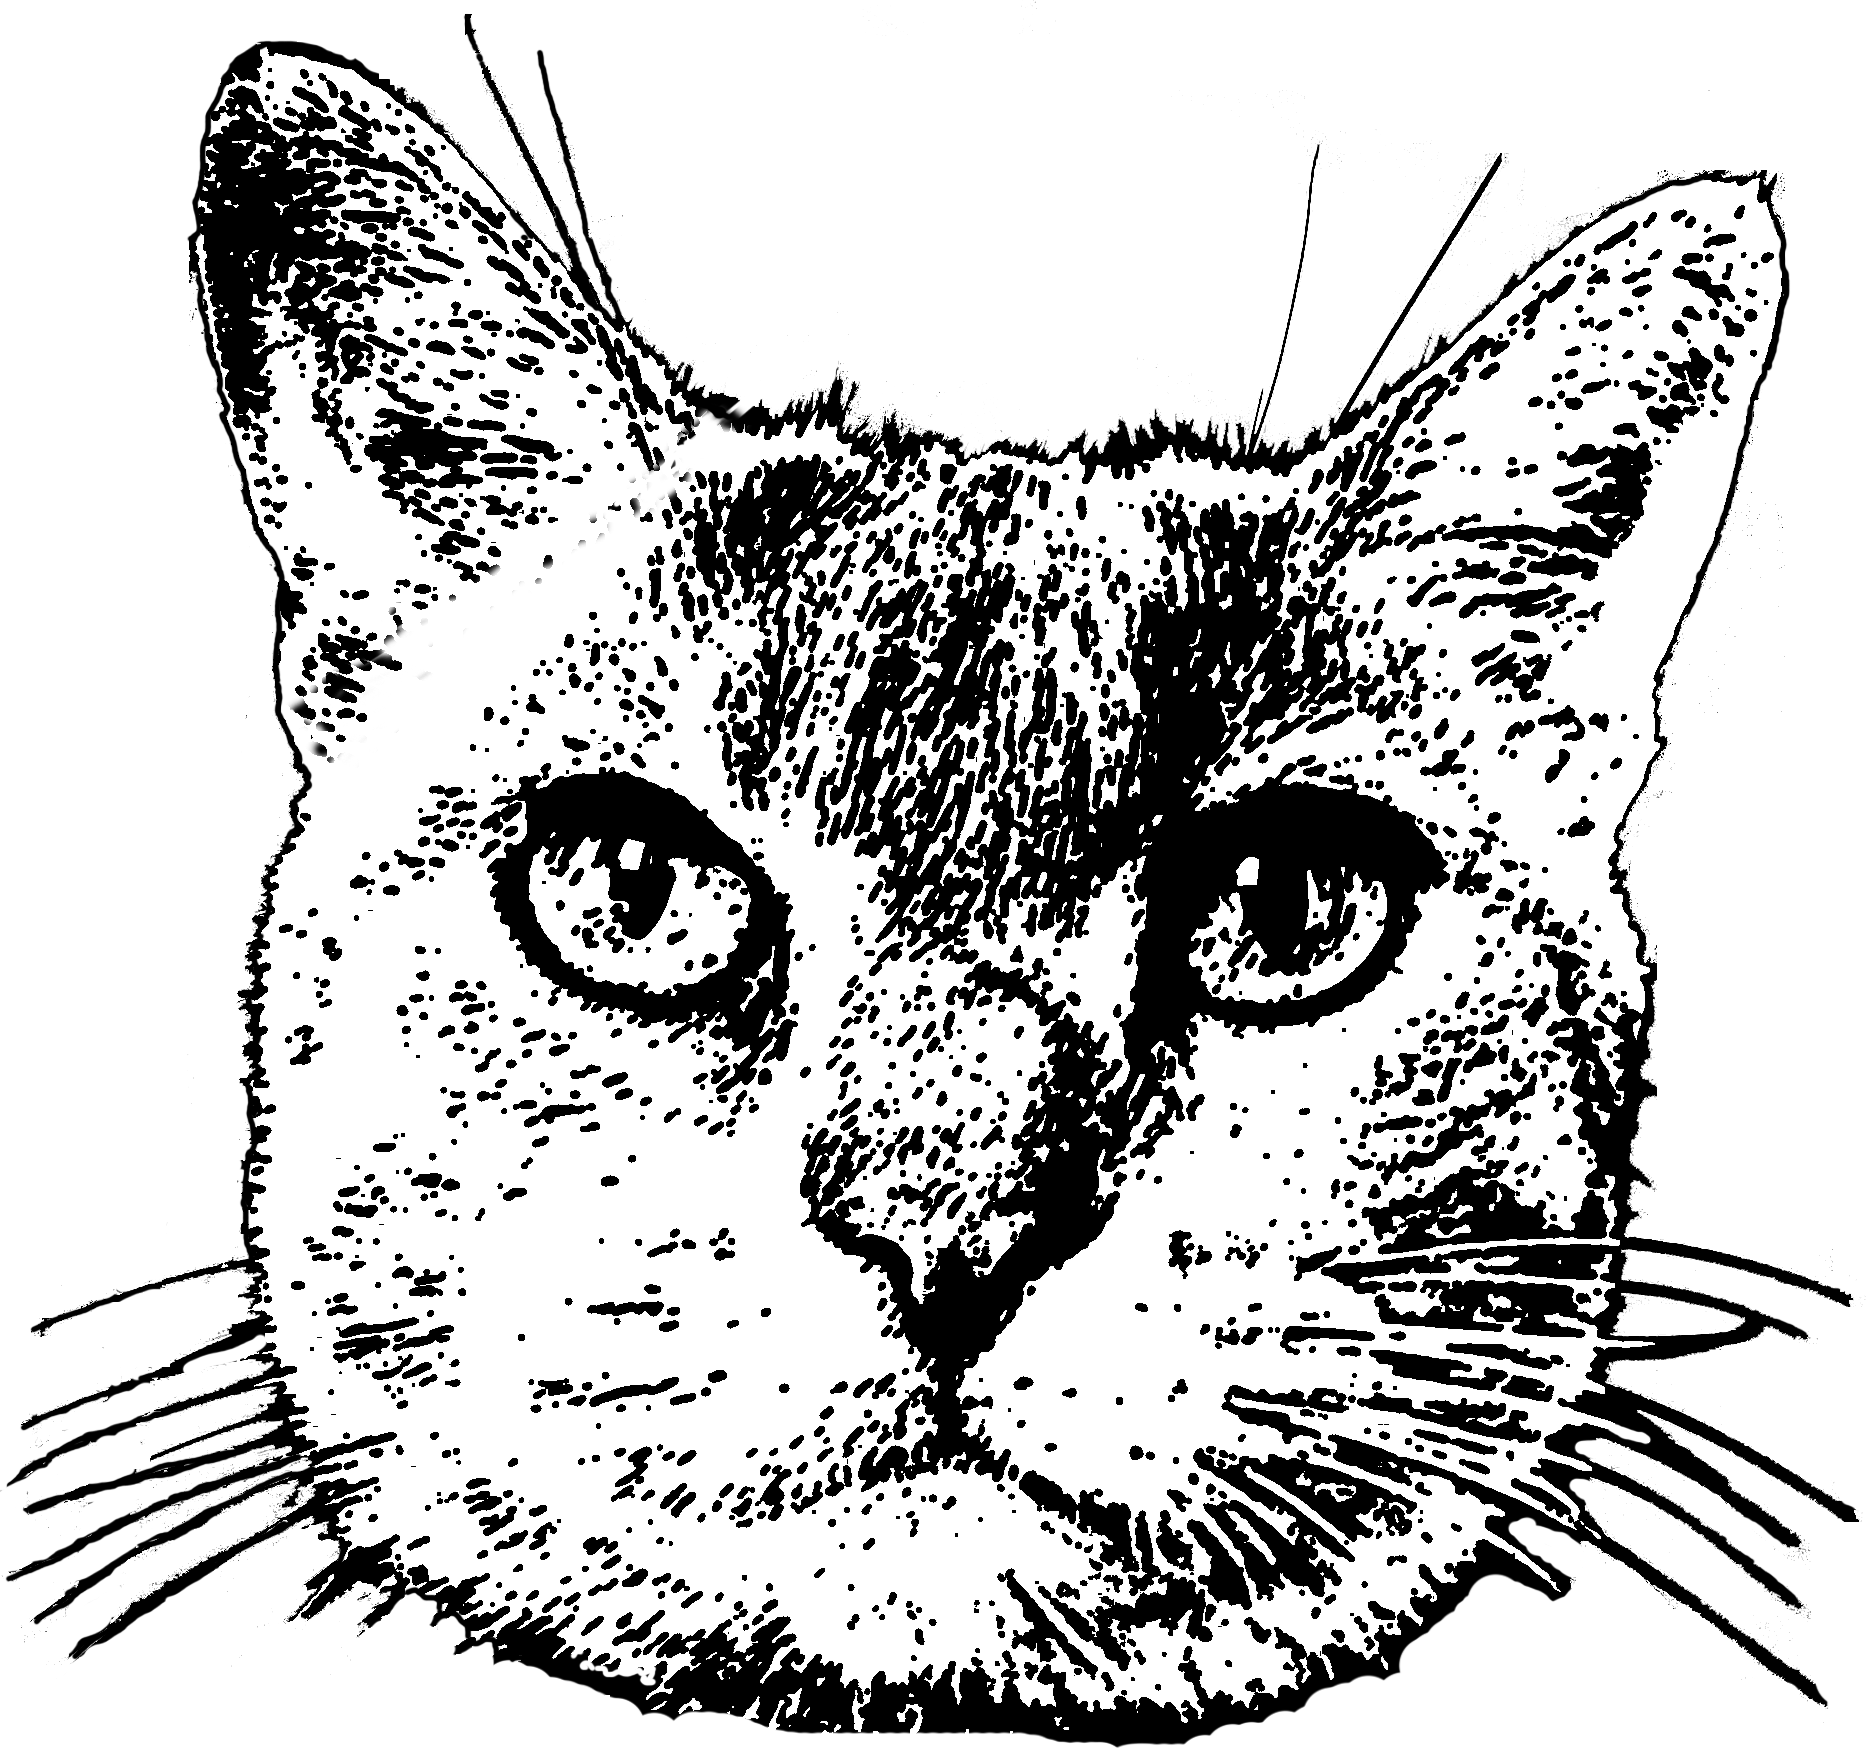
\includegraphics[width=0.1\textwidth]{keiko.png}}
	\rfoot{\thepage{}\hspace{1pt} van~\pageref{LastPage}}
	\lfoot{\tlpbox}


	\renewcommand{\headrulewidth}{0pt}

	\chead{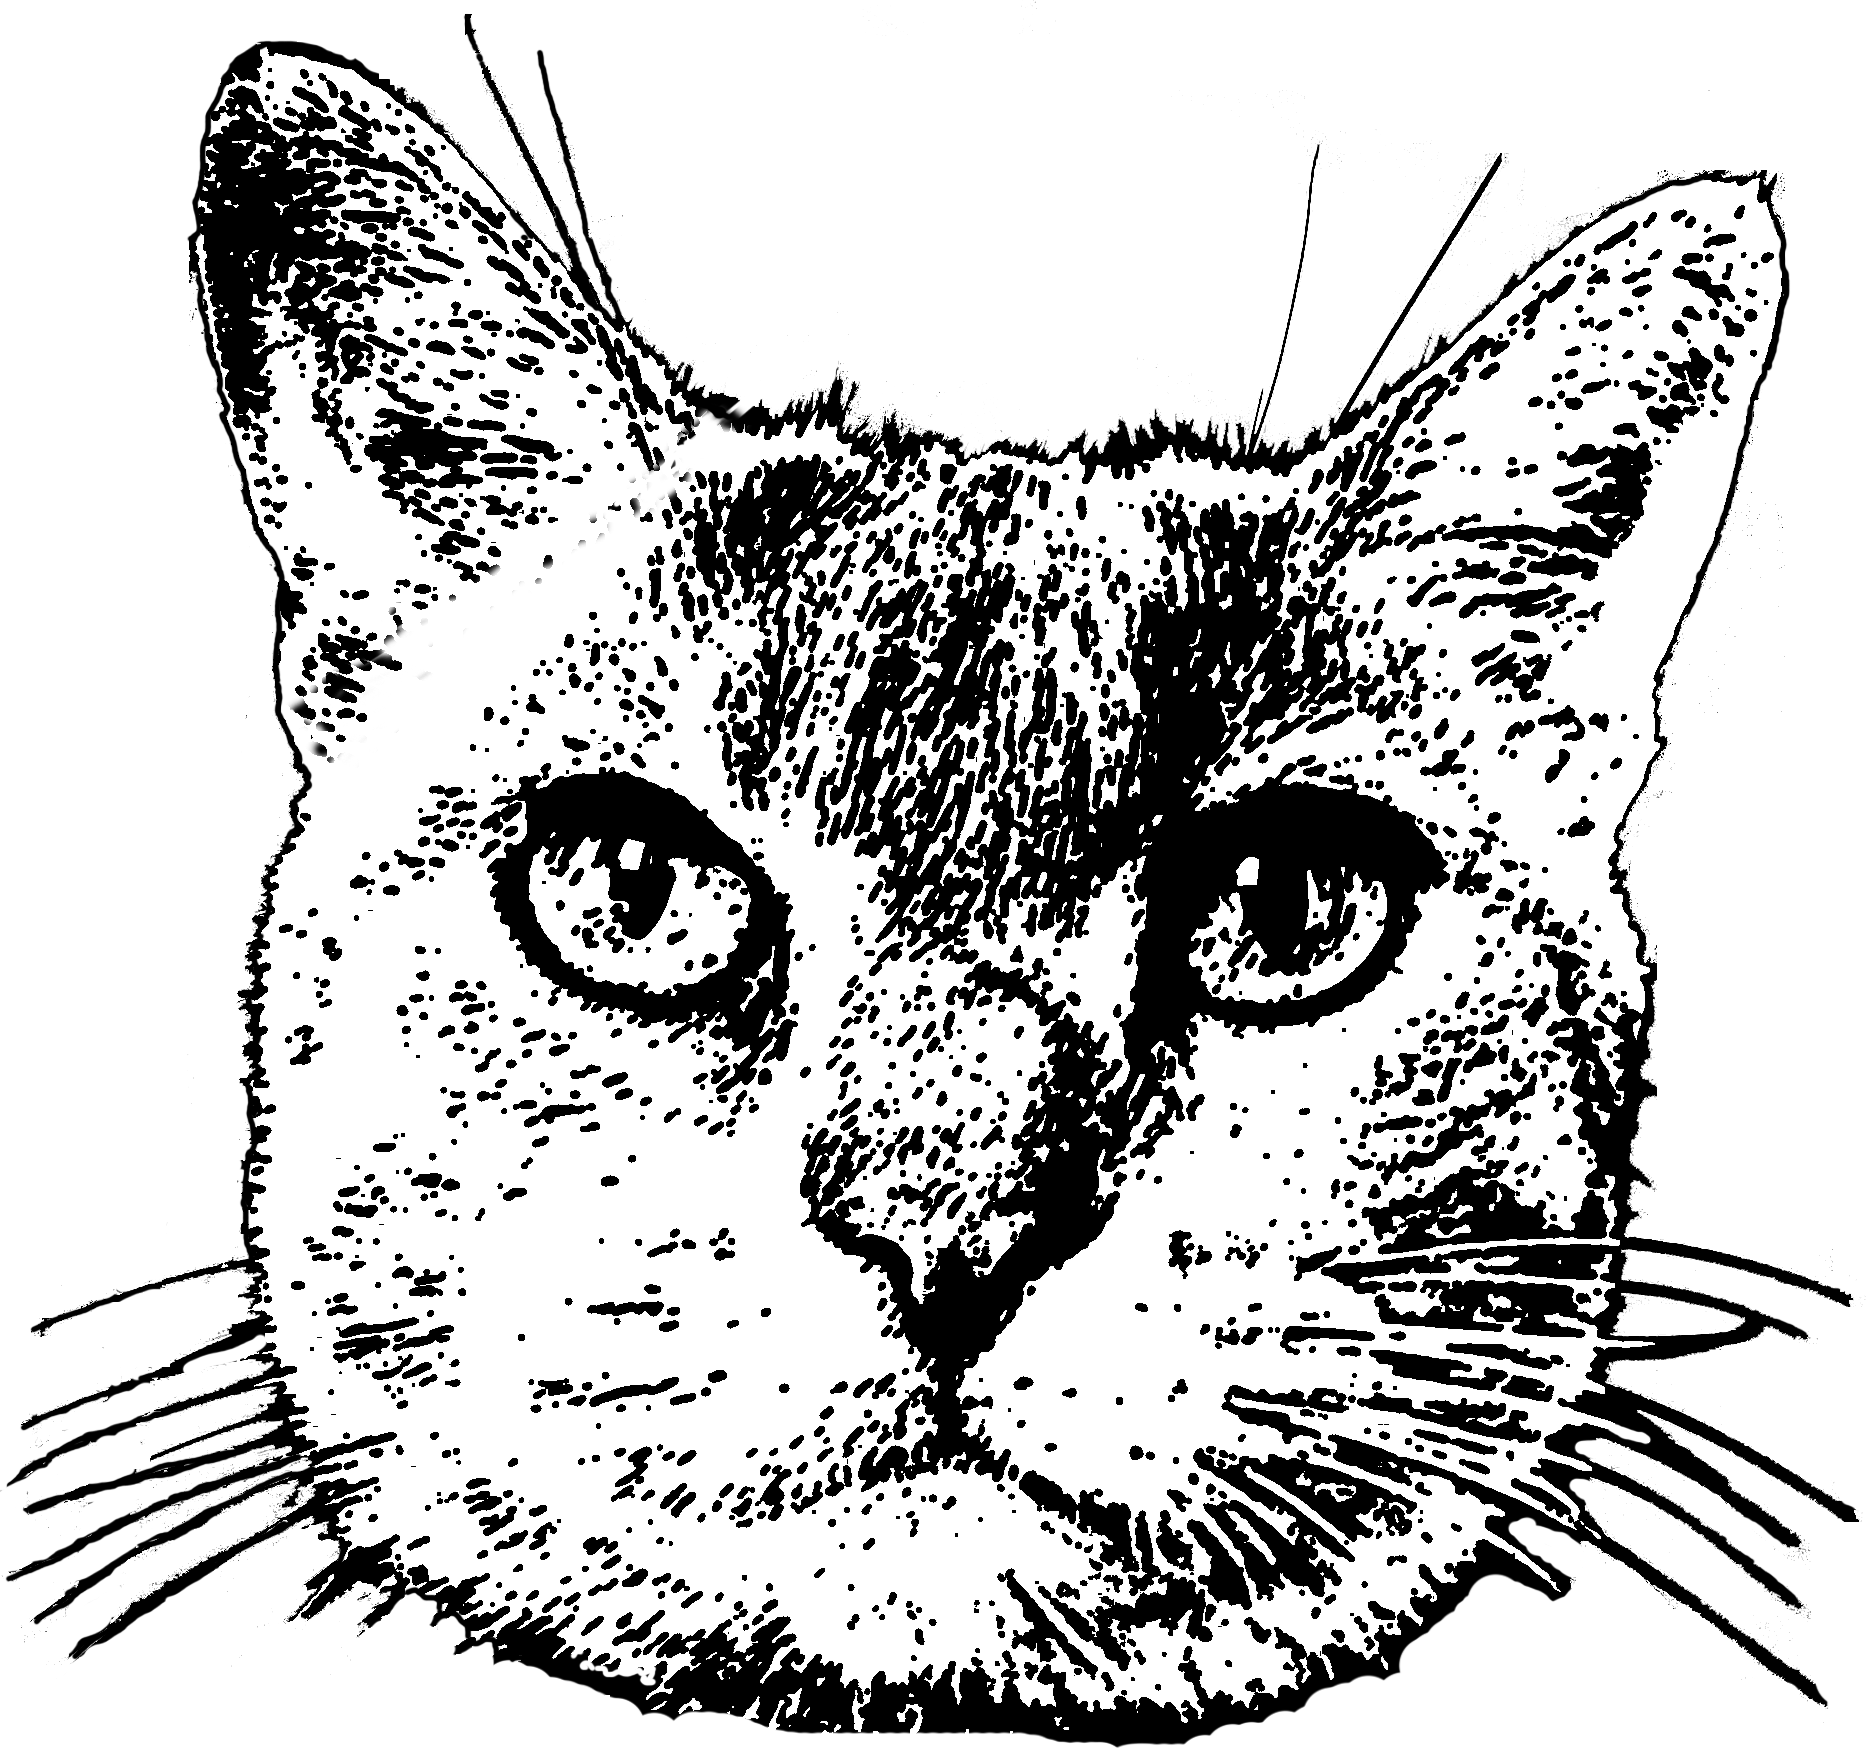
\includegraphics[width=0.05\textwidth]{keiko.png}}
	\lhead{\tlpbox}
	\rhead{\tlpbox}
	\renewcommand{\headrulewidth}{0pt}
}


% Title Page
\title{ \reporttitle{} }
\author{ \application{} }
\titlepic{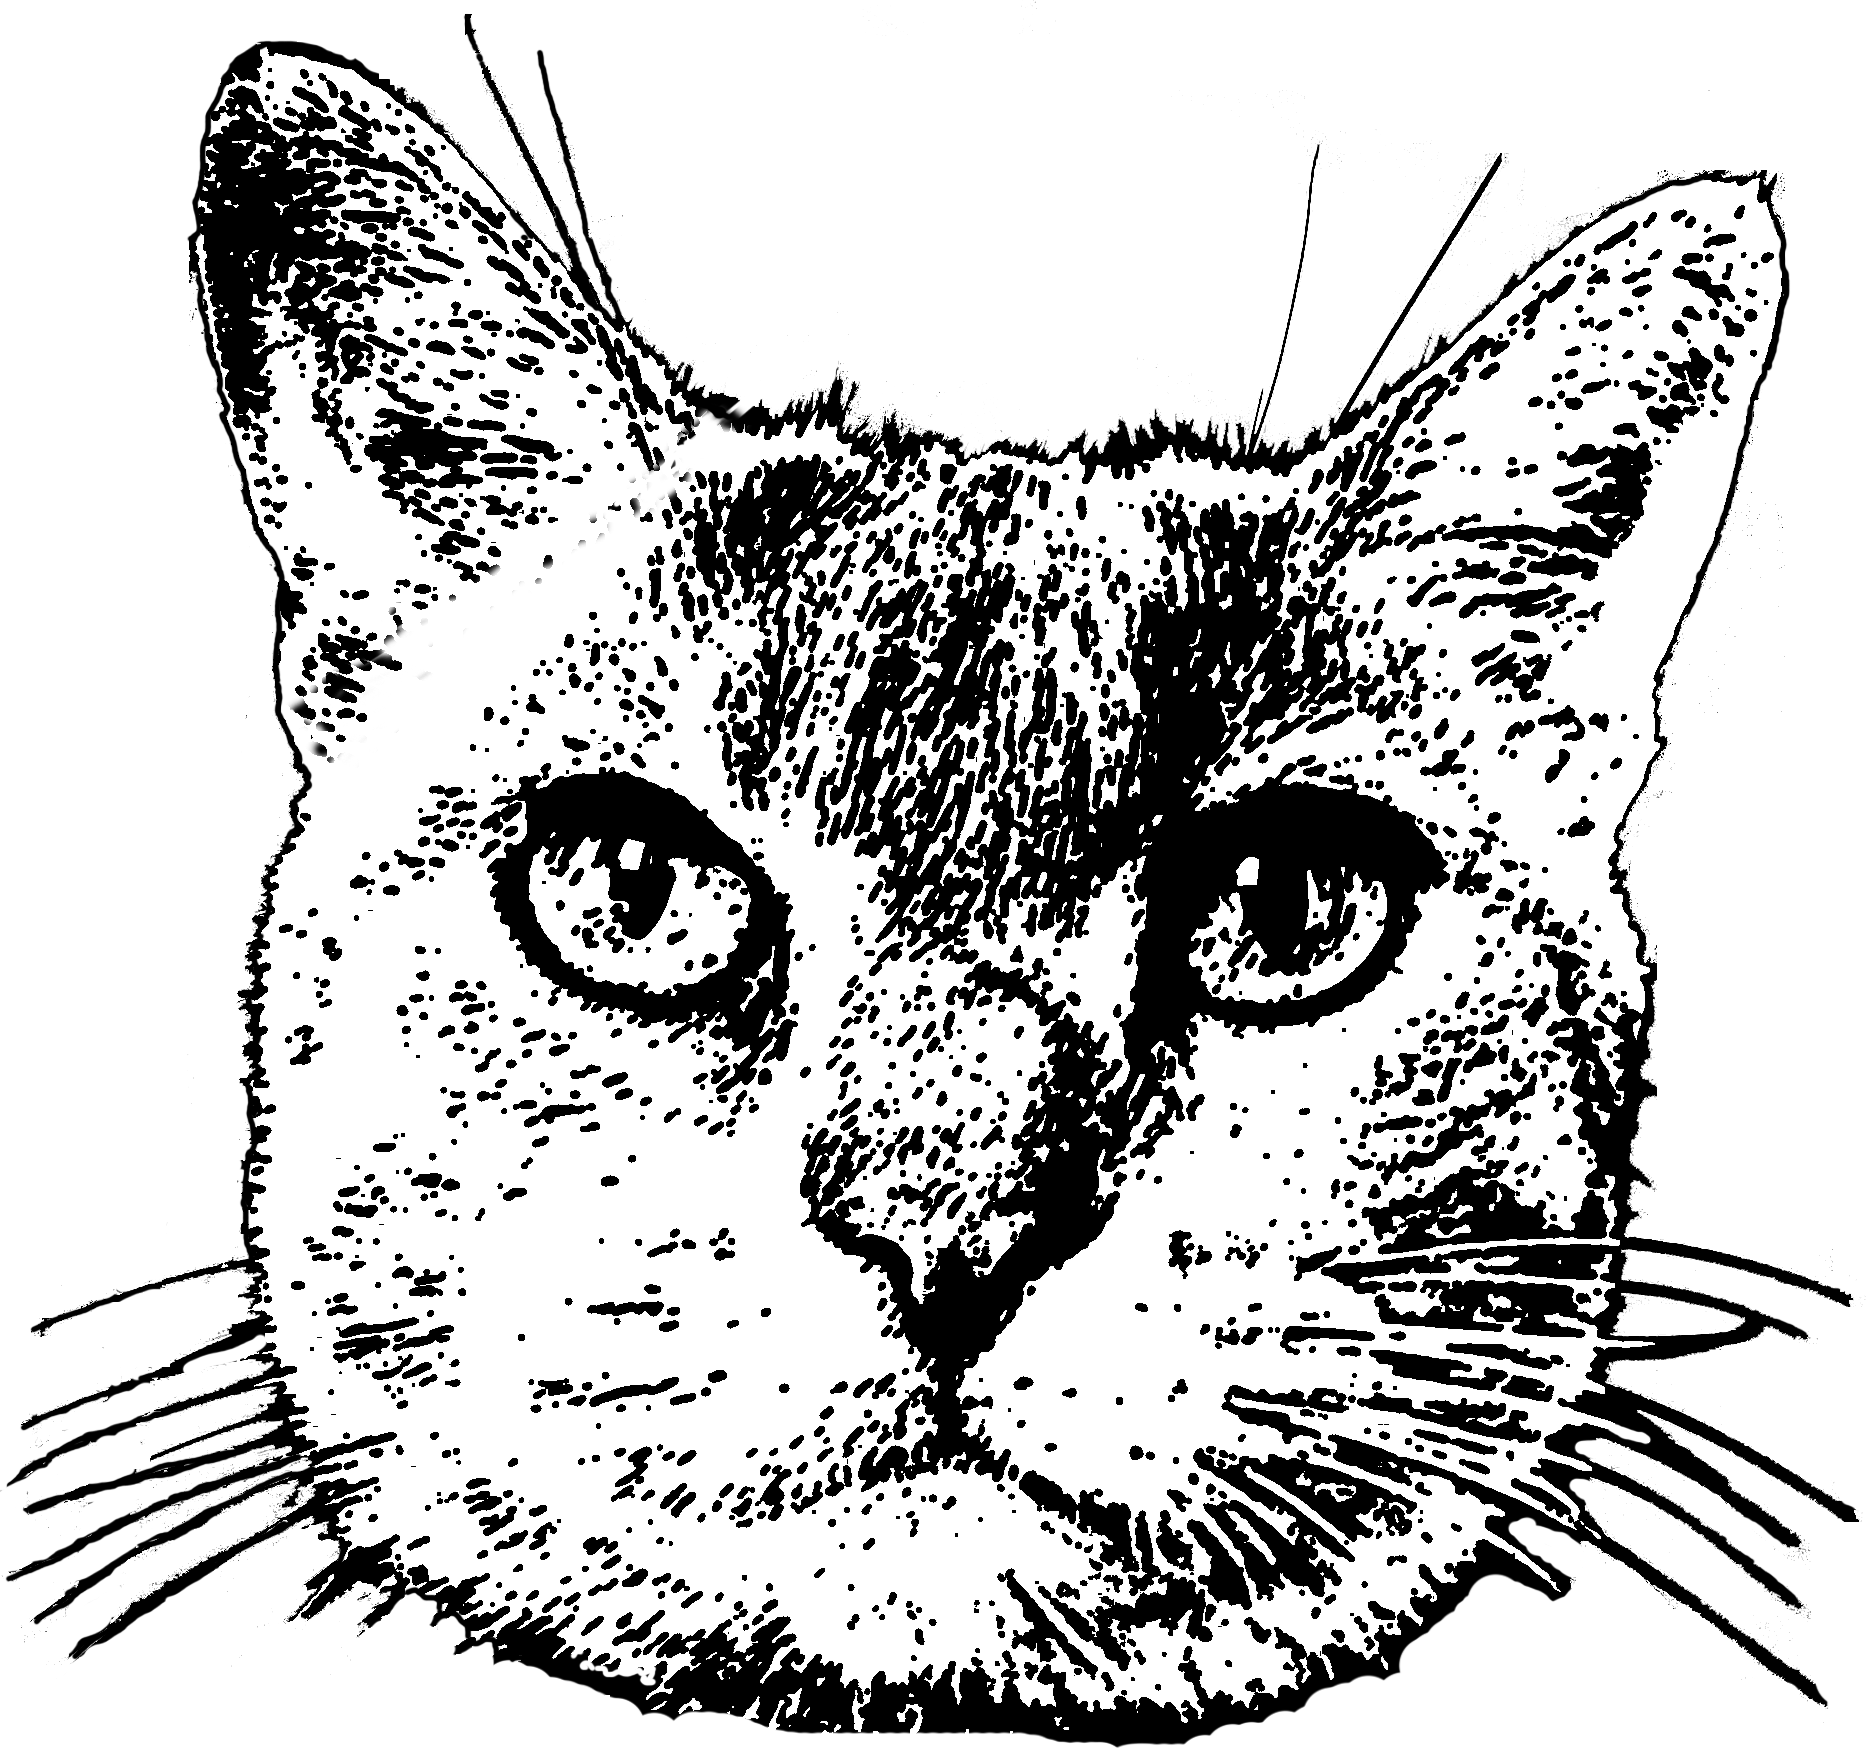
\includegraphics[width=70mm]{keiko.png}}

% To use a different font, uncomment the following lines.
% Run `fc-list` in the container to see which fonts are available.
%\usepackage{fontspec}
%\setmainfont{DejaVu Sans}

\begin{document}
\maketitle

\chapter{Over dit document}
\section{Vertrouwelijkheid}
In de informatiebeveiliging wordt gewerkt met het
\href{https://www.ncsc.nl/onderwerpen/traffic-light-protocol}{Traffic
Light Protocol (TLP)}. Dit is een internationale uniforme afspraak aan
de hand van de kleuren van het verkeerslicht. Het geeft aan hoe
vertrouwelijk informatie in het document is en of deze gedeeld mag
worden met andere personen of organisaties.

\begin{itemize}
     \item \colorbox{black}{\color{red}TLP:RED}. Deze informatie heeft
de hoogste vertrouwelijkheid. Deze mag niet met andere personen of
organisaties worden gedeeld. Vaak zal deze informatie mondeling worden
doorgegeven. In veel gevallen ook niet via e-mail of op papier, maar het
kan natuurlijk wel.
     \item \colorbox{black}{\color{orange}TLP:AMBER}. Deze informatie
mag op een need to know-basis worden gedeeld binnen de eigen organisatie
en de klanten (of aangesloten partijen).
     \item \colorbox{black}{\color{orange}TLP:AMBER+STRICT}. Deze
informatie mag alleen binnen de eigen organisatie worden gedeeld met
mensen voor wie toegang noodzakelijk is. Dit is op een `need to
know'-basis binnen de eigen organisatie.
     \item \colorbox{black}{\color{green}TLP:GREEN}. Deze informatie is
beschikbaar voor iedereen binnen de gemeenschap, waarop ze gericht is.
Dat betekent dat het nuttig kan zijn en daarmee gedeeld kan worden op
basis van `nice to know'. Er is geen restrictie tot de eigen organisatie.
     \item \colorbox{black}{\color{white}TLP:CLEAR}. Deze informatie is
niet vertrouwelijk en kan openbaar worden gedeeld.
\end{itemize}

\textbf{Dit document is gerubriceerd als \underline{TLP:\tlp}.}


\tableofcontents

\newpage

\chapter{Overzicht}

\section{Samenvatting}
Dit zijn de bevindingen van een OpenKAT-analyse op 2024-02-08 23:02:59 UTC. % chktex 36 chktex 18
De volgende filters zijn van toepassing op deze bevindingen:

\begin{longtable}{ p{.25\textwidth}  p{.75\textwidth} }

            Observed at & 2024{-}02{-}08 \\

            Severities &  \\

            Exclude muted & True \\

            Only muted & False \\

\end{longtable}



    \noindent Kopieer \href{http://localhost:8000/nl/_rieven/findings/?observed_at=2024-02-08}{deze link} om dit rapport te reproduceren.



\bgroup{}
\def\arraystretch{1.2}
\section{Totalen}
\begin{tabular}{ llr }
	Niveau & Uniek & Totaal aantal voorvallen \\\toprule
	\toprule

		\colorbox{box-color-critical}{ \color{color-critical} critical } & 0 & 0 \\

		\colorbox{box-color-high}{ \color{color-high} high } & 0 & 0 \\

		\colorbox{box-color-medium}{ \color{color-medium} medium } & 11 & 29 \\

		\colorbox{box-color-low}{ \color{color-low} low } & 3 & 13 \\

		\colorbox{box-color-recommendation}{ \color{color-recommendation} recommendation } & 1 & 4 \\

		\colorbox{box-color-pending}{ \color{color-pending} pending } & 1 & 1 \\

		\colorbox{box-color-unknown}{ \color{color-unknown} unknown } & 0 & 0 \\

	\bottomrule
	Totaal & 16 & 47
\end{tabular}
\egroup{}

\bgroup{}
\def\arraystretch{1.2}
\section{Bevinding types}
\resizebox{\columnwidth}{!}{
\begin{tabular}{ llr }
	Risico niveau & Bevindingstype & Voorvallen \\\toprule
	\midrule

		\colorbox{box-color-medium}{ \color{color-medium} medium } & KAT-NO-DKIM & 1 \\

		\colorbox{box-color-medium}{ \color{color-medium} medium } & KAT-NO-DMARC & 3 \\

		\colorbox{box-color-medium}{ \color{color-medium} medium } & KAT-NO-DNSSEC & 10 \\

		\colorbox{box-color-medium}{ \color{color-medium} medium } & KAT-NO-SPF & 1 \\

		\colorbox{box-color-medium}{ \color{color-medium} medium } & RetireJS-jquerymigrate-f3a3 & 2 \\

		\colorbox{box-color-medium}{ \color{color-medium} medium } & RetireJS-jquerymigrate-f901 & 2 \\

		\colorbox{box-color-medium}{ \color{color-medium} medium } & CVE-2016-10735 & 2 \\

		\colorbox{box-color-medium}{ \color{color-medium} medium } & CVE-2018-14040 & 2 \\

		\colorbox{box-color-medium}{ \color{color-medium} medium } & CVE-2018-14041 & 2 \\

		\colorbox{box-color-medium}{ \color{color-medium} medium } & CVE-2018-14042 & 2 \\

		\colorbox{box-color-medium}{ \color{color-medium} medium } & CVE-2019-8331 & 2 \\

		\colorbox{box-color-low}{ \color{color-low} low } & KAT-INVALID-RPKI & 8 \\

		\colorbox{box-color-low}{ \color{color-low} low } & KAT-NO-RPKI & 1 \\

		\colorbox{box-color-low}{ \color{color-low} low } & KAT-WEBSERVER-NO-IPV6 & 4 \\

		\colorbox{box-color-pending}{ \color{color-pending} pending } & KAT-EXPIRED-RPKI & 1 \\

		\colorbox{box-color-recommendation}{ \color{color-recommendation} recommendation } & KAT-NAMESERVER-NO-IPV6 & 4 \\

	\bottomrule
\end{tabular}}
\egroup{}


\chapter{Bevindingen}

	\section{KAT{-}NO{-}DKIM}
	\subsection{Bevinding informatie}
	\begin{longtable}{ p{.25\textwidth}  p{.75\textwidth} }
		Bevinding & KAT{-}NO{-}DKIM \\
		Risico niveau & 6.9 / 10 \\

		Ernst & Medium \\

		  Beschrijving & This hostname does not support a DKIM record. \\



			Aanbeveling & Set a DKIM record to protect your domain. \\



	\end{longtable}

	\subsection{Voorvallen}

		\subsubsection{\humanreadable{Hostname|internet|mispo.es}}
		This hostname does not support DKIM records



	\section{KAT{-}NO{-}DMARC}
	\subsection{Bevinding informatie}
	\begin{longtable}{ p{.25\textwidth}  p{.75\textwidth} }
		Bevinding & KAT{-}NO{-}DMARC \\
		Risico niveau & 6.9 / 10 \\

		Ernst & Medium \\

		  Beschrijving & This hostname does not have a DMARC record. \\



			Aanbeveling & Set a DMARC record to protect your domain. \\



	\end{longtable}

	\subsection{Voorvallen}

		\subsubsection{\humanreadable{Hostname|internet|domaindiscount24.net}}
		This hostname does not have a DMARC record

		\subsubsection{\humanreadable{Hostname|internet|mispo.es}}
		This hostname does not have a DMARC record

		\subsubsection{\humanreadable{Hostname|internet|rieven.com}}
		This hostname does not have a DMARC record



	\section{KAT{-}NO{-}DNSSEC}
	\subsection{Bevinding informatie}
	\begin{longtable}{ p{.25\textwidth}  p{.75\textwidth} }
		Bevinding & KAT{-}NO{-}DNSSEC \\
		Risico niveau & 6.9 / 10 \\

		Ernst & Medium \\

		  Beschrijving & The provided domain does not have DNSSEC enabled. \\



			Aanbeveling & Enable DNSSEC on your name servers. \\



	\end{longtable}

	\subsection{Voorvallen}

		\subsubsection{\humanreadable{Hostname|internet|domaindiscount24.net}}
		Domain domaindiscount24.net is not signed with DNSSEC.

		\subsubsection{\humanreadable{Hostname|internet|mispo.es}}
		Domain mispo.es is not signed with DNSSEC.

		\subsubsection{\humanreadable{Hostname|internet|ngrane.com}}
		Domain ngrane.com is not signed with DNSSEC.

		\subsubsection{\humanreadable{Hostname|internet|ns1.domaindiscount24.net}}
		Domain ns1.domaindiscount24.net is not signed with DNSSEC.

		\subsubsection{\humanreadable{Hostname|internet|ns1.ngrane.com}}
		Domain ns1.ngrane.com is not signed with DNSSEC.

		\subsubsection{\humanreadable{Hostname|internet|ns2.domaindiscount24.net}}
		Domain ns2.domaindiscount24.net is not signed with DNSSEC.

		\subsubsection{\humanreadable{Hostname|internet|ns2.ngrane.com}}
		Domain ns2.ngrane.com is not signed with DNSSEC.

		\subsubsection{\humanreadable{Hostname|internet|ns3.domaindiscount24.net}}
		Domain ns3.domaindiscount24.net is not signed with DNSSEC.

		\subsubsection{\humanreadable{Hostname|internet|rieven.com}}
		Domain rieven.com is not signed with DNSSEC.

		\subsubsection{\humanreadable{Hostname|internet|www.mispo.es}}
		Domain www.mispo.es is not signed with DNSSEC.



	\section{KAT{-}NO{-}SPF}
	\subsection{Bevinding informatie}
	\begin{longtable}{ p{.25\textwidth}  p{.75\textwidth} }
		Bevinding & KAT{-}NO{-}SPF \\
		Risico niveau & 6.9 / 10 \\

		Ernst & Medium \\

		  Beschrijving & This hostname does not have an SPF record. \\



			Aanbeveling & Set an SPF record to protect your domain. \\



	\end{longtable}

	\subsection{Voorvallen}

		\subsubsection{\humanreadable{Hostname|internet|mispo.es}}
		This hostname does not have an SPF record



	\section{RetireJS{-}jquerymigrate{-}f3a3}
	\subsection{Bevinding informatie}
	\begin{longtable}{ p{.25\textwidth}  p{.75\textwidth} }
		Bevinding & RetireJS{-}jquerymigrate{-}f3a3 \\
		Risico niveau & 6.9 / 10 \\

		Ernst & Medium \\

		  Beschrijving & cross{-}site{-}scripting. More information at: http://blog.jquery.com/2013/05/01/jquery{-}migrate{-}1{-}2{-}0{-}released/ or https://github.com/jquery/jquery{-}migrate/issues/36 \\





	\end{longtable}

	\subsection{Voorvallen}

		\subsubsection{\humanreadable{SoftwareInstance|HostnameHTTPURL|https|internet|mispo.es|443|/|Software|jQuery Migrate|1.0.0|}}
		This JavaScript Library has known vulnerabilities

		\subsubsection{\humanreadable{SoftwareInstance|HostnameHTTPURL|https|internet|www.mispo.es|443|/|Software|jQuery Migrate|1.0.0|}}
		This JavaScript Library has known vulnerabilities



	\section{RetireJS{-}jquerymigrate{-}f901}
	\subsection{Bevinding informatie}
	\begin{longtable}{ p{.25\textwidth}  p{.75\textwidth} }
		Bevinding & RetireJS{-}jquerymigrate{-}f901 \\
		Risico niveau & 6.9 / 10 \\

		Ernst & Medium \\

		  Beschrijving & Selector interpreted as HTML. More information at: http://bugs.jquery.com/ticket/11290 or http://research.insecurelabs.org/jquery/test/ \\





	\end{longtable}

	\subsection{Voorvallen}

		\subsubsection{\humanreadable{SoftwareInstance|HostnameHTTPURL|https|internet|mispo.es|443|/|Software|jQuery Migrate|1.0.0|}}
		This JavaScript Library has known vulnerabilities

		\subsubsection{\humanreadable{SoftwareInstance|HostnameHTTPURL|https|internet|www.mispo.es|443|/|Software|jQuery Migrate|1.0.0|}}
		This JavaScript Library has known vulnerabilities



	\section{CVE{-}2016{-}10735}
	\subsection{Bevinding informatie}
	\begin{longtable}{ p{.25\textwidth}  p{.75\textwidth} }
		Bevinding & CVE{-}2016{-}10735 \\
		Risico niveau & 6.1 / 10 \\

		Ernst & Medium \\

		  Beschrijving & In Bootstrap 3.x before 3.4.0 and 4.x{-}beta before 4.0.0{-}beta.2, XSS is possible in the data{-}target attribute, a different vulnerability than CVE{-}2018{-}14041. \\




			Bron& \href{https://cve.circl.lu/cve/CVE{-}2016{-}10735}{https://cve.circl.lu/cve/CVE{-}2016{-}10735} \\


	\end{longtable}

	\subsection{Voorvallen}

		\subsubsection{\humanreadable{SoftwareInstance|HostnameHTTPURL|https|internet|mispo.es|443|/|Software|Bootstrap|3.3.7|cpe:/a:getbootstrap:bootstrap}}
		This JavaScript Library has known vulnerabilities

		\subsubsection{\humanreadable{SoftwareInstance|HostnameHTTPURL|https|internet|www.mispo.es|443|/|Software|Bootstrap|3.3.7|cpe:/a:getbootstrap:bootstrap}}
		This JavaScript Library has known vulnerabilities



	\section{CVE{-}2018{-}14040}
	\subsection{Bevinding informatie}
	\begin{longtable}{ p{.25\textwidth}  p{.75\textwidth} }
		Bevinding & CVE{-}2018{-}14040 \\
		Risico niveau & 6.1 / 10 \\

		Ernst & Medium \\

		  Beschrijving & In Bootstrap before 4.1.2, XSS is possible in the collapse data{-}parent attribute. \\




			Bron& \href{https://cve.circl.lu/cve/CVE{-}2018{-}14040}{https://cve.circl.lu/cve/CVE{-}2018{-}14040} \\


	\end{longtable}

	\subsection{Voorvallen}

		\subsubsection{\humanreadable{SoftwareInstance|HostnameHTTPURL|https|internet|mispo.es|443|/|Software|Bootstrap|3.3.7|cpe:/a:getbootstrap:bootstrap}}
		This JavaScript Library has known vulnerabilities

		\subsubsection{\humanreadable{SoftwareInstance|HostnameHTTPURL|https|internet|www.mispo.es|443|/|Software|Bootstrap|3.3.7|cpe:/a:getbootstrap:bootstrap}}
		This JavaScript Library has known vulnerabilities



	\section{CVE{-}2018{-}14041}
	\subsection{Bevinding informatie}
	\begin{longtable}{ p{.25\textwidth}  p{.75\textwidth} }
		Bevinding & CVE{-}2018{-}14041 \\
		Risico niveau & 6.1 / 10 \\

		Ernst & Medium \\

		  Beschrijving & In Bootstrap before 4.1.2, XSS is possible in the data{-}target property of scrollspy. \\




			Bron& \href{https://cve.circl.lu/cve/CVE{-}2018{-}14041}{https://cve.circl.lu/cve/CVE{-}2018{-}14041} \\


	\end{longtable}

	\subsection{Voorvallen}

		\subsubsection{\humanreadable{SoftwareInstance|HostnameHTTPURL|https|internet|mispo.es|443|/|Software|Bootstrap|3.3.7|cpe:/a:getbootstrap:bootstrap}}
		This JavaScript Library has known vulnerabilities

		\subsubsection{\humanreadable{SoftwareInstance|HostnameHTTPURL|https|internet|www.mispo.es|443|/|Software|Bootstrap|3.3.7|cpe:/a:getbootstrap:bootstrap}}
		This JavaScript Library has known vulnerabilities



	\section{CVE{-}2018{-}14042}
	\subsection{Bevinding informatie}
	\begin{longtable}{ p{.25\textwidth}  p{.75\textwidth} }
		Bevinding & CVE{-}2018{-}14042 \\
		Risico niveau & 6.1 / 10 \\

		Ernst & Medium \\

		  Beschrijving & In Bootstrap before 4.1.2, XSS is possible in the data{-}container property of tooltip. \\




			Bron& \href{https://cve.circl.lu/cve/CVE{-}2018{-}14042}{https://cve.circl.lu/cve/CVE{-}2018{-}14042} \\


	\end{longtable}

	\subsection{Voorvallen}

		\subsubsection{\humanreadable{SoftwareInstance|HostnameHTTPURL|https|internet|mispo.es|443|/|Software|Bootstrap|3.3.7|cpe:/a:getbootstrap:bootstrap}}
		This JavaScript Library has known vulnerabilities

		\subsubsection{\humanreadable{SoftwareInstance|HostnameHTTPURL|https|internet|www.mispo.es|443|/|Software|Bootstrap|3.3.7|cpe:/a:getbootstrap:bootstrap}}
		This JavaScript Library has known vulnerabilities



	\section{CVE{-}2019{-}8331}
	\subsection{Bevinding informatie}
	\begin{longtable}{ p{.25\textwidth}  p{.75\textwidth} }
		Bevinding & CVE{-}2019{-}8331 \\
		Risico niveau & 6.1 / 10 \\

		Ernst & Medium \\

		  Beschrijving & In Bootstrap before 3.4.1 and 4.3.x before 4.3.1, XSS is possible in the tooltip or popover data{-}template attribute. \\




			Bron& \href{https://cve.circl.lu/cve/CVE{-}2019{-}8331}{https://cve.circl.lu/cve/CVE{-}2019{-}8331} \\


	\end{longtable}

	\subsection{Voorvallen}

		\subsubsection{\humanreadable{SoftwareInstance|HostnameHTTPURL|https|internet|mispo.es|443|/|Software|Bootstrap|3.3.7|cpe:/a:getbootstrap:bootstrap}}
		This JavaScript Library has known vulnerabilities

		\subsubsection{\humanreadable{SoftwareInstance|HostnameHTTPURL|https|internet|www.mispo.es|443|/|Software|Bootstrap|3.3.7|cpe:/a:getbootstrap:bootstrap}}
		This JavaScript Library has known vulnerabilities



	\section{KAT{-}INVALID{-}RPKI}
	\subsection{Bevinding informatie}
	\begin{longtable}{ p{.25\textwidth}  p{.75\textwidth} }
		Bevinding & KAT{-}INVALID{-}RPKI \\
		Risico niveau & 3.9 / 10 \\

		Ernst & Low \\

		  Beschrijving & The IP address does not have a valid route announcement that is matched by the published Route Policy and Authorization (RPKI) \\



			Aanbeveling & Make sure that the Route Origin Authorizations (ROAs) that specify which Autonomous Systems (AS) are authorized to announce your IP addresses are valid and not expired. \\



	\end{longtable}

	\subsection{Voorvallen}

		\subsubsection{\humanreadable{IPAddressV4|internet|109.234.111.81}}
		The IP address does not have a valid route announcement that is matched by the published Route Policy and Authorization (RPKI)

		\subsubsection{\humanreadable{IPAddressV4|internet|134.209.85.72}}
		The IP address does not have a valid route announcement that is matched by the published Route Policy and Authorization (RPKI)

		\subsubsection{\humanreadable{IPAddressV4|internet|144.217.35.18}}
		The IP address does not have a valid route announcement that is matched by the published Route Policy and Authorization (RPKI)

		\subsubsection{\humanreadable{IPAddressV4|internet|66.206.3.125}}
		The IP address does not have a valid route announcement that is matched by the published Route Policy and Authorization (RPKI)

		\subsubsection{\humanreadable{IPAddressV4|internet|94.23.153.36}}
		The IP address does not have a valid route announcement that is matched by the published Route Policy and Authorization (RPKI)

		\subsubsection{\humanreadable{IPAddressV6|internet|2001:41d0:c:388:94:23:153:36}}
		The IP address does not have a valid route announcement that is matched by the published Route Policy and Authorization (RPKI)

		\subsubsection{\humanreadable{IPAddressV6|internet|2604:4500:c:3:66:206:3:125}}
		The IP address does not have a valid route announcement that is matched by the published Route Policy and Authorization (RPKI)

		\subsubsection{\humanreadable{IPAddressV6|internet|2607:5300:60:5e1c:144:217:35:18}}
		The IP address does not have a valid route announcement that is matched by the published Route Policy and Authorization (RPKI)



	\section{KAT{-}NO{-}RPKI}
	\subsection{Bevinding informatie}
	\begin{longtable}{ p{.25\textwidth}  p{.75\textwidth} }
		Bevinding & KAT{-}NO{-}RPKI \\
		Risico niveau & 3.9 / 10 \\

		Ernst & Low \\

		  Beschrijving & The IP address does not have a route announcement that is matched by the published Route Policy and Authorization (RPKI) \\



			Aanbeveling & Work on implementing RPKI for your IP addresses. This may involve creating Route Origin Authorizations (ROAs) that specify which Autonomous Systems (AS) are authorized to announce your IP addresses. \\



	\end{longtable}

	\subsection{Voorvallen}

		\subsubsection{\humanreadable{IPAddressV4|internet|31.187.70.163}}
		The IP address does not have a route announcement that is matched by the published Route Policy and Authorization (RPKI)



	\section{KAT{-}WEBSERVER{-}NO{-}IPV6}
	\subsection{Bevinding informatie}
	\begin{longtable}{ p{.25\textwidth}  p{.75\textwidth} }
		Bevinding & KAT{-}WEBSERVER{-}NO{-}IPV6 \\
		Risico niveau & 3.9 / 10 \\

		Ernst & Low \\

		  Beschrijving & For this website there is no web server with an IPv6 address available. \\



			Aanbeveling & Add an IPv6 address for at least one web server that has no IPv6 address yet. \\



	\end{longtable}

	\subsection{Voorvallen}

		\subsubsection{\humanreadable{Hostname|internet|domaindiscount24.net}}
		There are no webservers with an IPv6 address.

		\subsubsection{\humanreadable{Hostname|internet|mispo.es}}
		There are no webservers with an IPv6 address.

		\subsubsection{\humanreadable{Hostname|internet|ngrane.com}}
		There are no webservers with an IPv6 address.

		\subsubsection{\humanreadable{Hostname|internet|rieven.com}}
		There are no webservers with an IPv6 address.



	\section{KAT{-}EXPIRED{-}RPKI}
	\subsection{Bevinding informatie}
	\begin{longtable}{ p{.25\textwidth}  p{.75\textwidth} }
		Bevinding & KAT{-}EXPIRED{-}RPKI \\
		Risico niveau & 0.0 / 10 \\

		Ernst & Pending \\





	\end{longtable}

	\subsection{Voorvallen}

		\subsubsection{\humanreadable{IPAddressV4|internet|31.187.70.163}}
		None



	\section{KAT{-}NAMESERVER{-}NO{-}IPV6}
	\subsection{Bevinding informatie}
	\begin{longtable}{ p{.25\textwidth}  p{.75\textwidth} }
		Bevinding & KAT{-}NAMESERVER{-}NO{-}IPV6 \\
		Risico niveau & 0.0 / 10 \\

		Ernst & Recommendation \\

		  Beschrijving & This nameserver does not have an ipv6 address. \\





	\end{longtable}

	\subsection{Voorvallen}

		\subsubsection{\humanreadable{DNSNSRecord|internet|ngrane.com|ns1.ngrane.com.}}
		This nameserver has no ipv6 address

		\subsubsection{\humanreadable{DNSNSRecord|internet|ngrane.com|ns2.ngrane.com.}}
		This nameserver has no ipv6 address

		\subsubsection{\humanreadable{DNSNSRecord|internet|rieven.com|ns1.ngrane.com.}}
		This nameserver has no ipv6 address

		\subsubsection{\humanreadable{DNSNSRecord|internet|rieven.com|ns2.ngrane.com.}}
		This nameserver has no ipv6 address





\chapter{Verklarende Woordenlijst}
\begin{longtable}{ p{.25\textwidth}  p{.75\textwidth} } \toprule
	\textbf{Begrip} & \textbf{Betekenis} \\\toprule \endhead{}

		CVSS & Common Vulnerability Scoring System. Systeem om een score te geven aan een zwakke plek in soft - ware. Hoe hoger de score, hoe zwakker de plek. Een organisatie kan deze score gebruiken om te bepalen welke zwakke plekken ze als eerste gaat oplossen. Meer informatie over het scoresysteem staat op \\href{https://www.first.org/cvss/}. \\ \midrule

		Document & Er zijn in de wetgeving twee definities van een document, die beiden duidelijk maken dat in de juridische zin een document iedere vorm van informatie is, zoals een schriftelijk stuk, e-mail, social media bericht, database, enzovoort. In de Wet op de parlementaire enquete is een document in artikel 1, eerste lid onder c gedefinieerd als Schriftelijk stuk of ander materiaal dat gegevens bevat. In de Wet open overheid is dit in artikel 2, eerste lid gedefinieerd als:
document: een door een orgaan, persoon of college als bedoeld in artikel 2.2, eerste lid, opgemaakt of ontvangen schriftelijk stuk of ander geheel van vastgelegde gegevens dat naar zijn aard verband houdt met de publieke taak van dat orgaan, die persoon of dat college; \\ \midrule

		Informatiebeveiliging & Alles wat men doet om ervoor te zorgen dat men bij informatie kan komen wanneer men dat wil, dat de informatie klopt en dat de informatie niet bij anderen terecht komt. Het gaat daarbij vaak om een computersysteem, maar dat hoeft niet. Het gaat om maatregelen, procedures en processen die beveiligingsproblemen voorkomen, opsporen, onderdrukken en oplossen. Ontstaat er wel een probleem met de informatie? Dan zorgt informatiebeveiliging ervoor dat de gevolgen zoveel mogelijk beperkt worden.  \\ \midrule

		Risico & Kans op schade of verlies in een computersysteem, gecombineerd met de gevolgen die deze schade heeft voor de organisatie. Een voorbeeld van schade kan bijvoorbeeld zijn dat mensen informatie zien die ze niet hadden mogen zien. Of dat men niet meer zeker weet of gegevens nog kloppen. Bij gevolgen voor de organisatie kan men denken aan financiële schade of het verlies van de goede naam van de organisatie. \\ \midrule

		TLP & Traffic Light Protocol. Een methode om data of informatie in te delen in klasses. Hoe men dit indeelt, hangt af van met wie men de informatie mag delen. De klasses zijn rood, oranje, groen en wit. \\ \midrule

		Vertrouwelijkheid & Informatie is vertrouwelijk als het alleen gezien wordt door iemand die het gegeven ook mag zien. Degene die het gegeven maakt, bepaalt wie het mag zien. Vertrouwelijkheid is een van de kwaliteitskenmerken van gegevens. \\ \midrule

	\bottomrule
\end{longtable}

\end{document}
